\documentclass[12pt]{article} 
%\usepackage{fullpage} %full page typesetting
\usepackage{setspace} %allows for non-singlespacing
\usepackage{graphicx} %graphics capabilities
\usepackage{latexsym} %extra symbols
\usepackage{rotating} %rotation for figures
\usepackage{longtable} %tables that fill more than a single page
\usepackage{footnote} %footnotes
\usepackage{hyperref} %hypertext links in the document
\usepackage{natbib} %better bibliographies
\usepackage{authblk} %author and affiliation in opening
\usepackage{mathpazo} %use palatino font, rather than times

\title{Benefit Threat to City Solvency}
\author{Cheikhou Kane, Faith Benamy, and Jack Reilly}
%\href{mailto:citysolvency@ncf.edu}{\nolinkurl{citysolvency@ncf.edu}}}
%\date{5/1/2020}
\affil{New College of Florida}
\doublespacing 
\newcommand\e{\emph}
\newcommand\tb{\textbf}
\newcommand\un{\underline}
\begin{document}
\begin{singlespace} 

\maketitle

~\\\\\\\\\\\\\\\\\\\\\\\\\\\\\\\\\

\begin{center}
 \e{Correspondence or Questions: citysolvency@ncf.edu} \\
 \e{Working paper draft, please do not cite or quote without permission}\\
 \e{Contributions: Study design, writing, graphics (CK, FB, JR); ~~~~~~~~~~~~~~~~~~~~~~~~~~~~~~data collection and analysis (CK, FB)}\\ ~\\
  \e{Acknowledgements: The authors thank Robert Pozen and the New College of Florida Data Science Program for support and feedback on this report}
\end{center}
\thispagestyle{empty} 

\end{singlespace} 

\clearpage

\begin{center} 
\section*{Executive Summary}

\begin{quote}
	

The unfunded obligations of the pension and other post employment
benefits (OPEB) plans sponsored by local governments in the United
States continue to grow. In the following report, we study in detail the
financial obligations of 21 of the 22 largest US cities (excluding
Washington, DC, the 20th largest city). We review both their own reports
on these obligations and how these differ from our estimates based on
more realistic assumptions.

~~~~~We find that most cities reported OPEB liabilities close to our
measures, however, for pensions, we find that cities drastically
undervalue their unfunded liabilities. In fact, at the end of the 2017
fiscal year, these largest U.S. cities reported unfunded liabilities of
approximately \textbf{\$545} billion: \textbf{\$432} billion for
pensions and \textbf{\$113} billion for OPEB. According to our
calculations, we estimate the true unfunded liabilities to be over
\textbf{\$803} billion: \textbf{\$672} billion for pensions and
\textbf{\$131} billion for OPEB.

~~~~~The largest discrepancy, between the unfunded pension liabilities
reported by the cities and our estimates of their pension liabilities,
is primarily the result of different discount rates used in valuing
these liabilities. Under government accounting standards, cities are
given broad discretion to choose a discount rate based on their
expectation of future returns on plan assets. Thus, there is wide
variation in the discount rate chosen by cities in their reporting, with
several cities choosing highly optimistic discount rates for their
pension plans at 7\% or higher (see Appendix).

~~~~~But discount rates are supposed to represent a conservative rate of
return with a high degree of confidence. For example, the FASB %Financial Accounting Standards Board
stipulates that corporations must use the AA corporate bond rate as the
discount rate for their pension plans. In June, 2017, the AA corporate
bond rate for 15 years was approximately 4\%. Therefore, we used that
4\% as the discount rate in our estimates of the unfunded liabilities
for pensions in all 21 cities, and a 3\% discount rate for OPEBs to
account for the comparably shorter liabilities of OPEBs relative to
pensions.

~~~~~Our report is divided into three main parts. First, we present in
detail the unfunded pension liability of the 21 cities, followed by
pension liability per capita and pension liability as a percentage of
revenues. Second, we present in detail the unfunded OPEB liability of
the cities, followed by OPEB liability per capital and OPEB liability
as a percentage of revenues. Third, we present total pension and OPEB
liabilities for each city, followed by total liabilities per capita and
as share of revenue. 

\end{quote}

\end{center}

\section{Pension Liability}

In this section, we study in detail the pension liability of the 21
cities. We report on both the city's own calculations of their pension
obligations, based on their Comprehensive Annual Financial Reports
(CAFRs), and illustrate how these differ from valuations using a
standardized discount rate calculation. First, we present the total
unfunded pension liability for each city in dollars. Second, we showcase
the total liability scaled by population size. Finally, we present the
2017 pension expense as a share of governmental fund revenues.


\subsection{Total Pension
Liability}

The difference in the reported pension liability and the ones calculated
under our standardized valuation are illustrated in Figure 1 below. In
general, the higher discount rates used by cities in their calculations
result in much lower - sometimes, dramatically lower - estimates of
their unfunded liabilities, with cities like New York, Los Angeles, and
Chicago reporting particularly extreme total differences. Even cities
without extreme values generally report a value notably lower than the
standardized value, with only Fort Worth reporting an unfunded pension
liability close to our standardized measure.

\begin{figure}
  \makebox[\textwidth][c]{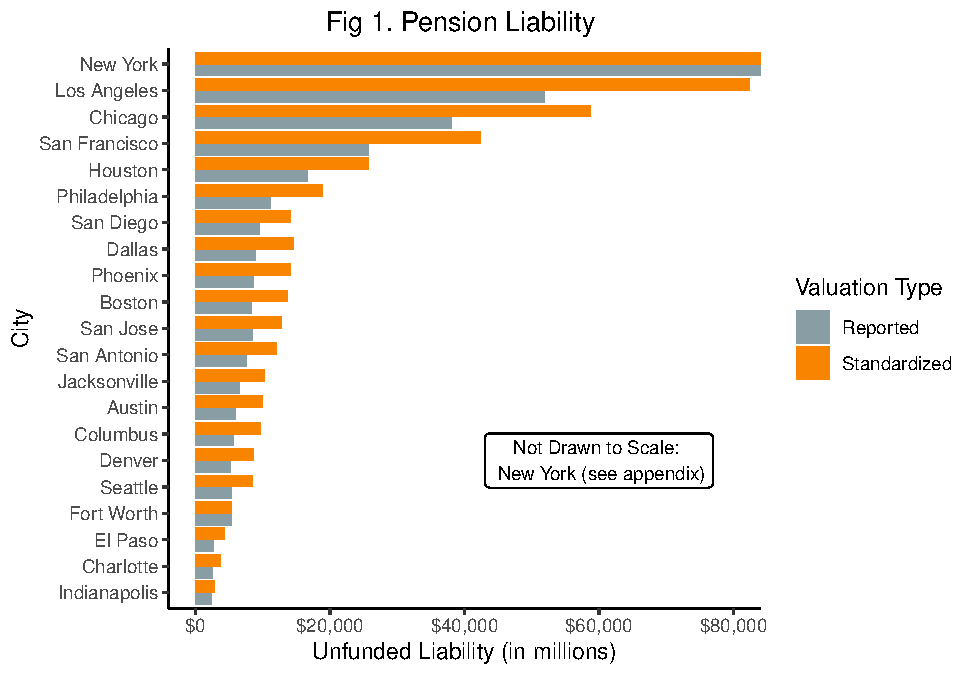
\includegraphics[width=1.2\textwidth]{City-Solvency-Report--Adjusted-_files/figure-latex/unnamed-chunk-6-1.pdf}}%
  %\caption{Caption}
  \label{fig:key}
\end{figure}

%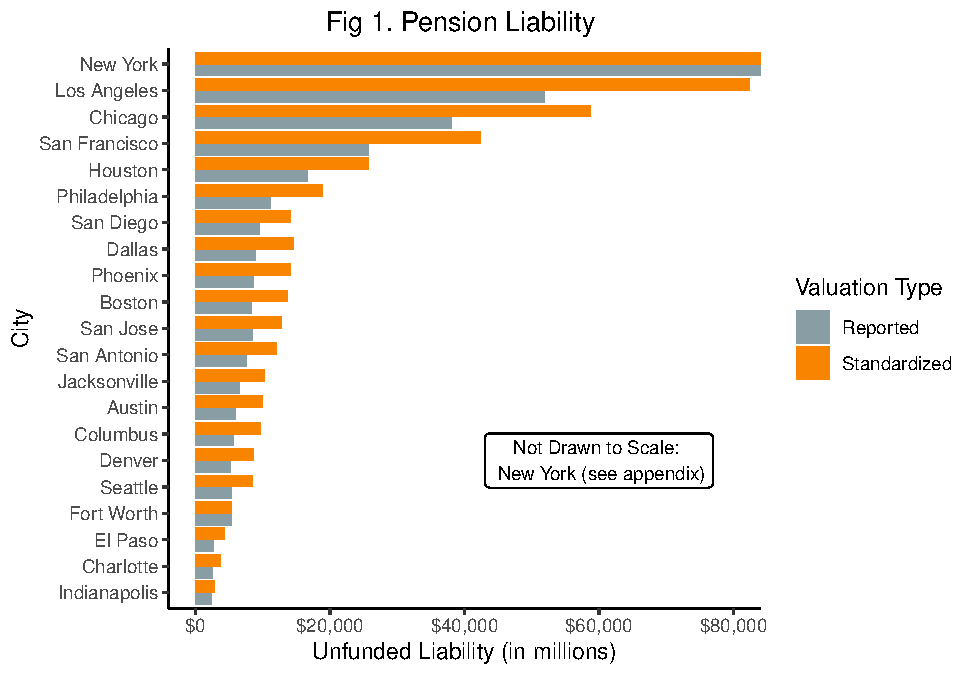
\includegraphics{City-Solvency-Report--Adjusted-_files/figure-latex/unnamed-chunk-6-1.pdf}

\subsection{Total Pension Liability Per
Capita}

To better illustrate the scale of concern for unfunded pension
liability, we provide per capita measures to represent a city's pension
financial burden relative to their population size (see Figure 2). This also allows
comparisons with other cities more naturally. As before, city
obligations were under-reported in reported city CAFR values, with an average
reported total pension liability per capita of \textbf{\$8,934}. In comparison, we calculated the average standardized total pension liability per capita to be
\textbf{\$14,035}.

\begin{figure}
  \makebox[\textwidth][c]{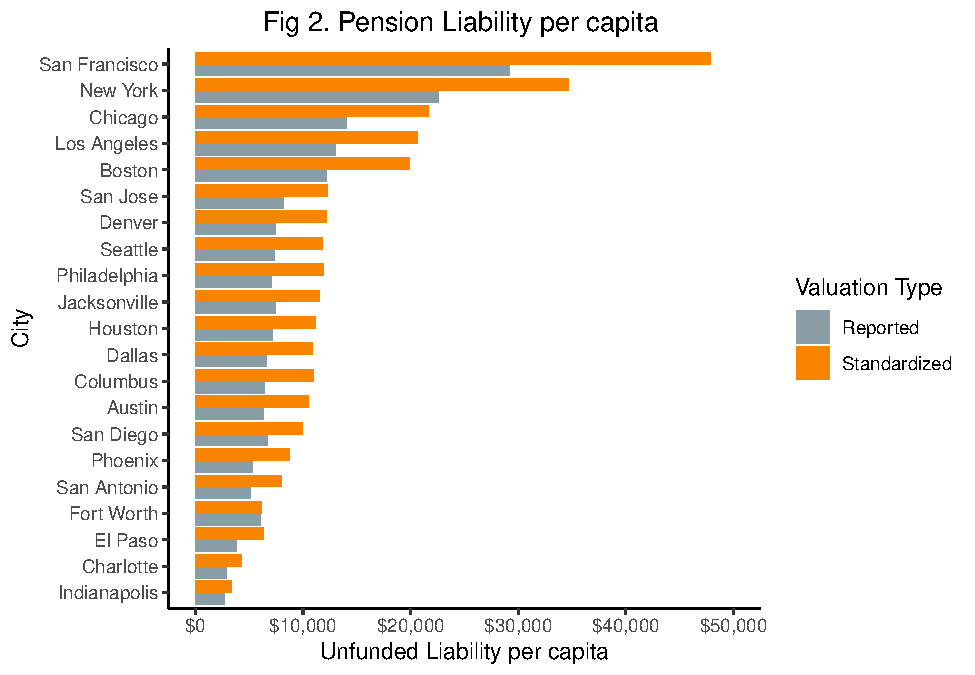
\includegraphics[width=1.2\textwidth]{City-Solvency-Report--Adjusted-_files/figure-latex/unnamed-chunk-7-1.pdf}}%
  %\caption{Caption}
  \label{fig:key}
\end{figure}

Furthermore, the variation in city obligation becomes clearer, as some
cities appear to be in more extreme fiscal danger while others appear to
have more manageable situations, relative to their populations (and
thus, potential tax base). As before, Fort Worth has little difference
between their reported and standardized values as well as the lowest
total unfunded obligation per capita. While New York has the largest
unfunded pension liability in terms of total dollar amount, the massive
scale of the city's population moves it further down the list here.

\subsection{Share of Revenue}

Finally, city's reported pension expense as a share of a city's governmental fund revenues is illustrated in Figure 3.
This provides another view into city management of pension fund
obligations, with significant variation in city share of revenue. On average, share of revenue was
\textbf{33.13\%} with a low of \textbf{0.85\%} for Seattle and a high of
\textbf{73.64\%} for Dallas.

\begin{figure}
  \makebox[\textwidth][c]{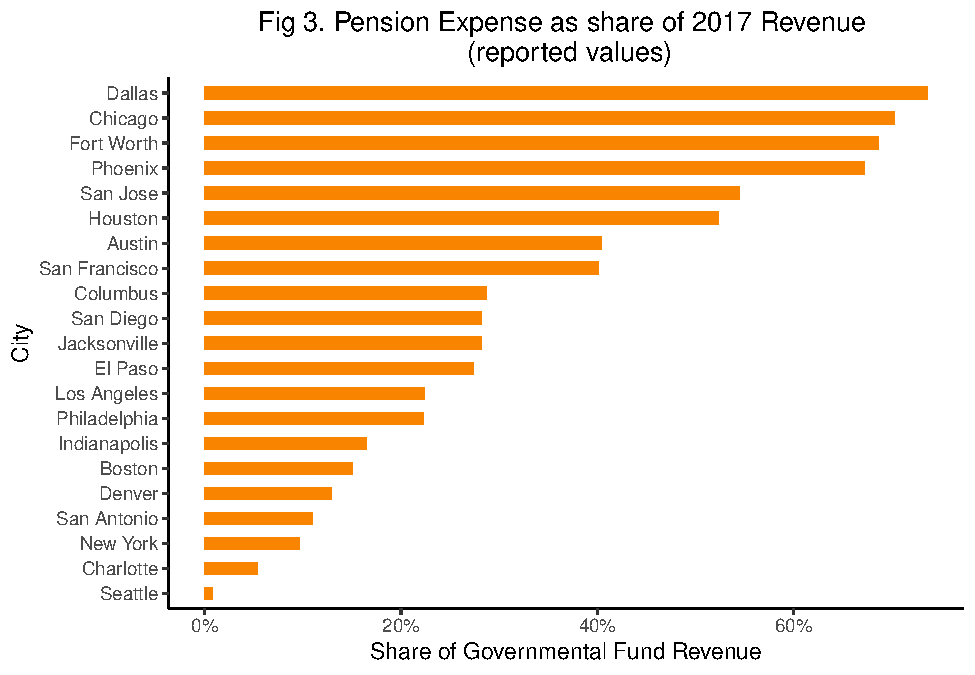
\includegraphics[width=1.2\textwidth]{City-Solvency-Report--Adjusted-_files/figure-latex/unnamed-chunk-8-1.pdf}}%
  %\caption{Caption}
  \label{fig:key}
\end{figure}

\section{OPEB Liability}

In this section, we evaluate the other post employment benefit (OPEB)
liability of cities in our study.\footnote{While Columbus was included in our pension numbers, we exclude it here, due to it taking part in a statewide OPEB plan.} As before, we report on both a city's
own calculations of their OPEB obligations and how these differ from
valuations using a standardized measure with consistent and appropriately conservative discount rate
assumptions. In addition, we provide several ways of evaluation city
financial burden due to OPEB.

First, we present the total Unfunded Actuarial Accrued Liability
(the UAAL) - the difference between the present value of benefit payment
(current and past) and the present value of the OPEB Asset Fund. Second,
we showcase the total UAAL scaled by population size. Finally, we
present the share of each city's revenue utilized to cover OPEB benefit
payments.


\subsection{Unfunded OPEB
Liability}

The difference in the reported UAALs and the ones calculated under our
standardized valuation are illustrated in Figure 4 below. As before,
most cities report lower unfunded liabilities than more reasonable
discount rate assumptions would suggest.

\begin{figure}
  \makebox[\textwidth][c]{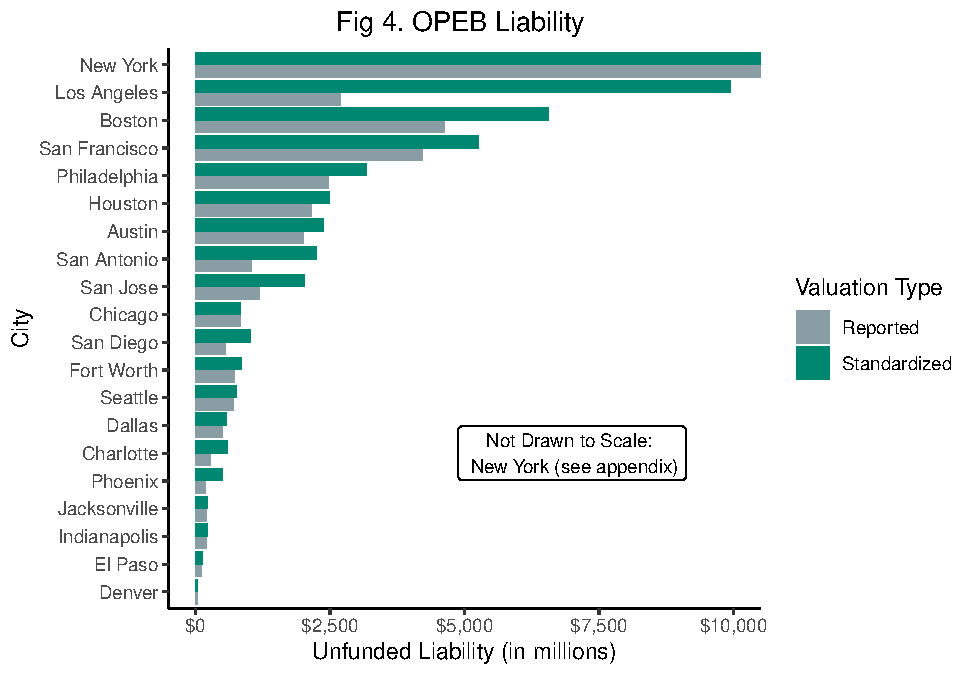
\includegraphics[width=1.2\textwidth]{City-Solvency-Report--Adjusted-_files/figure-latex/unnamed-chunk-9-1.pdf}}%
  %\caption{Caption}
  \label{fig:key}
\end{figure}

Also as expected, cities with the larger populations (e.g., New York, Los
Angeles) tend to carry the highest amounts of unfunded obligations,
although there is little correlation between the actual size of city's
obligations and the extent to which they proportionately underestimate
those obligations. While Los Angeles has a dramatic difference between
actual and reported values, so do cities further down the scale, such as
San Antonio, Charlotte, and Phoenix. 

\subsection{Unfunded OPEB Liability Per
Capita}

The difference in the reported UAALs and our own valuations scaled by
population size are illustrated in Figure 5 below. As before, this
allows for an arguably clearer indication of a city's fiscal status.

In addition to allowing for greater comparability between cities in
OPEB, such scale allows for greater comparability with city pension
obligations as well. One thing that obviously arises is how much more
sizable pension liability is when compared to OPEB liability. While there are some
liability values near \$10,000, the median per capita OPEB liability is
well under \$5,000, with all but a few cities illustrating obligations
(even by standardized reporting) under \$3,000 per capita and many under
\$1,000. This compares to average standardized obligations of approximately \$14,000 per person per city in the pension arena. We also note that there is not
necessarily a clear relation between OPEB obligation and pension
obligation - while Denver, for example, is at bottom in regards to
their OPEB liability, in regards to pensions, they are further up the
list.


\begin{figure}
  \makebox[\textwidth][c]{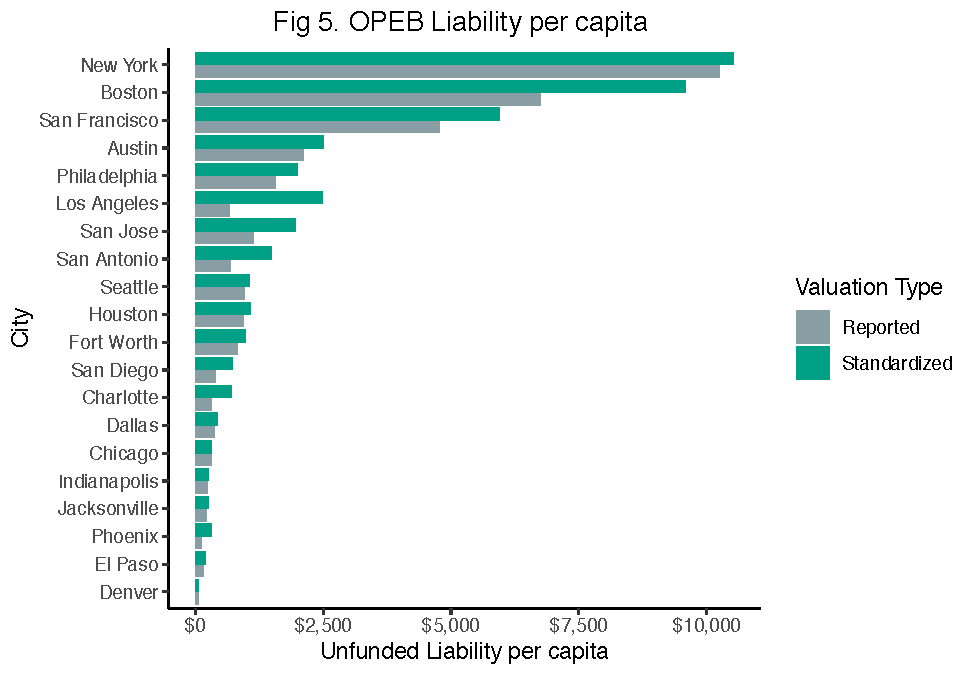
\includegraphics[width=1.2\textwidth]{City-Solvency-Report--Adjusted-_files/figure-latex/unnamed-chunk-10-1.pdf}}%
  %\caption{Caption}
  \label{fig:key}
\end{figure}


\subsection{Share of revenue}

OPEB payments as a share of a city's revenues in 2017 is illustrated in Figure 6. This further provides users
with another alternative to compare cities regarding their OPEB
financial burden. The average share of revenue was \textbf{2.95\%} with
a low of \textbf{0.16\%} for Denver and a high of \textbf{7.2\%} for Los
Angeles. 

\begin{figure}
  \makebox[\textwidth][c]{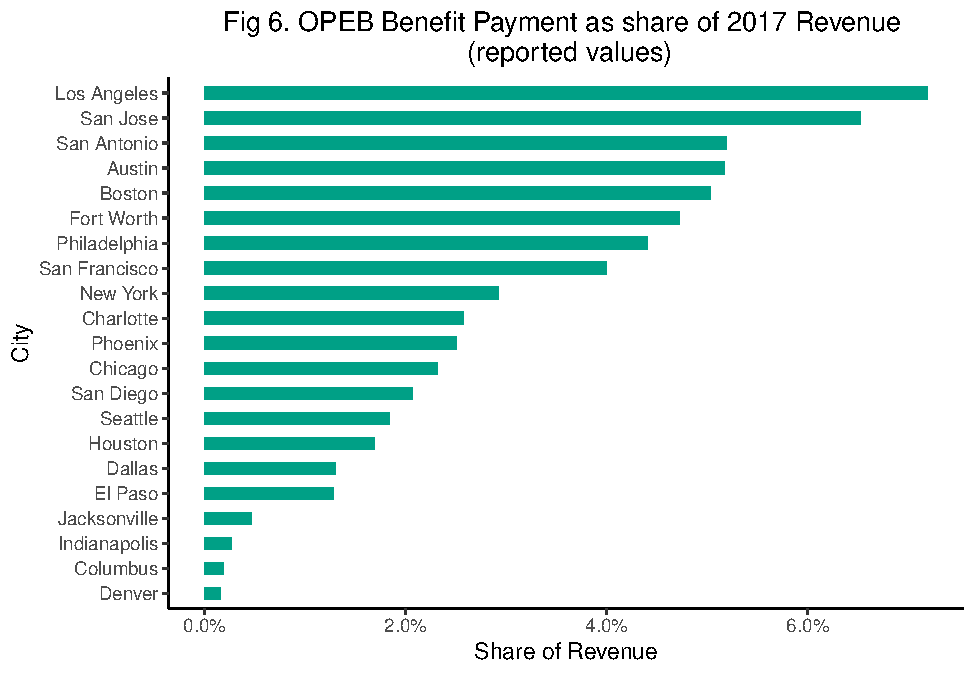
\includegraphics[width=1.2\textwidth]{City-Solvency-Report--Adjusted-_files/figure-latex/unnamed-chunk-11-1.pdf}}%
  %\caption{Caption}
  \label{fig:key}
\end{figure}


\section{Total Unfunded Liability}

In this section, we combine our results from the two previous sections
to study in detail the total unfunded liability of the cities in
question. We report on both their own estimates of their total
obligations as well as a standardized measure. As before, we first
present the total unfunded liability in dollar terms, then showcase the
total liability scaled by population size, and finally display payments
as share of revenue.


\subsection{Total Unfunded Liability}

The difference in the total city reported liability (pension and OPEB
combined) and the standardized valuation we calculate is illustrated in
Figure 7 below. Unsurprisingly, for all cities, the standardized total
liability is greater than the reported value. The average reported total
liability was about \textbf{\$27} billion per city while the average
standardized total liability was around \textbf{\$40} billion per city,
with larger cities logically under greater burdens.

\begin{figure}
  \makebox[\textwidth][c]{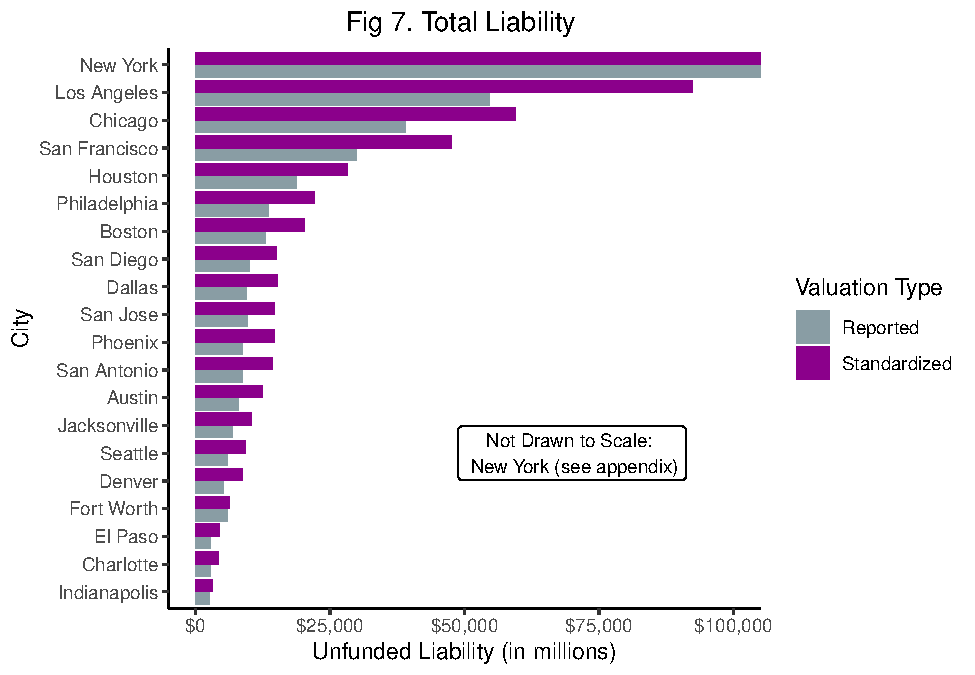
\includegraphics[width=1.2\textwidth]{City-Solvency-Report--Adjusted-_files/figure-latex/unnamed-chunk-12-1.pdf}}%
  %\caption{Caption}
  \label{fig:key}
\end{figure}


\subsection{Total Unfunded Liability Per
Capita}

Figure 8 below shows the total liability per capita for all the cities
included in our report. As before, the total unfunded liabilities these
cities reported were usually lower than our standardized measures, but
the per capita measure allows for a different comparison. In particular,
we note how these numbers are primarily driven by pension numbers, where
obligations tend to be larger.

\begin{figure}
  \makebox[\textwidth][c]{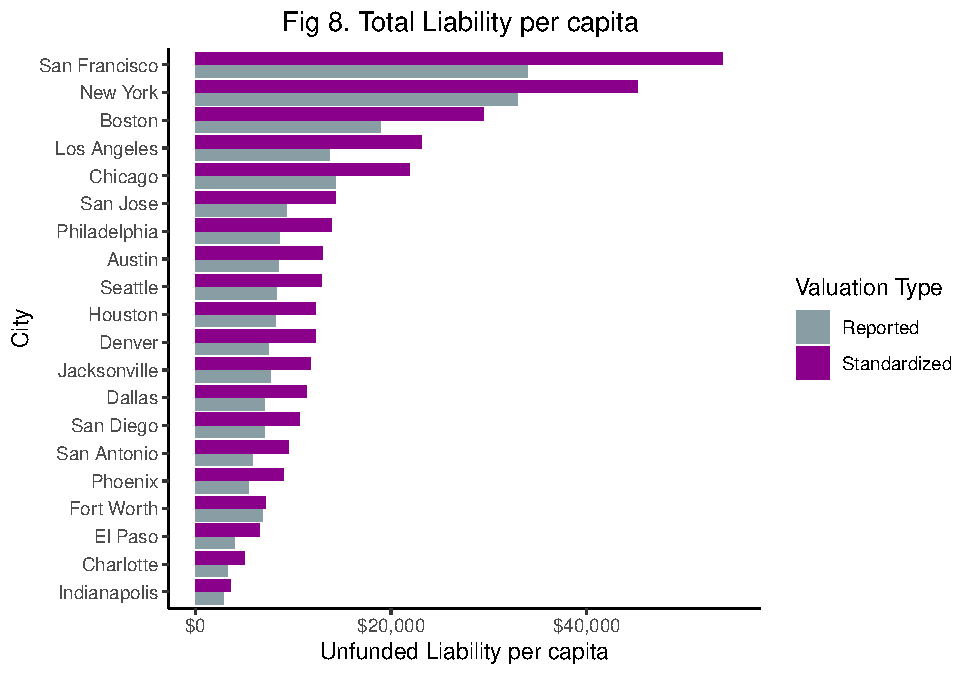
\includegraphics[width=1.2\textwidth]{City-Solvency-Report--Adjusted-_files/figure-latex/unnamed-chunk-13-1.pdf}}%
  %\caption{Caption}
  \label{fig:key}
\end{figure}

\subsection{City Pension and OPEB Payments and Expenses as share
Revenue}

Finally, Figure 9 reports overall city pension and OPEB payments and expenses
as a share of revenue, which again illustrates significant diversity
among cities' payments.

\begin{figure}
  \makebox[\textwidth][c]{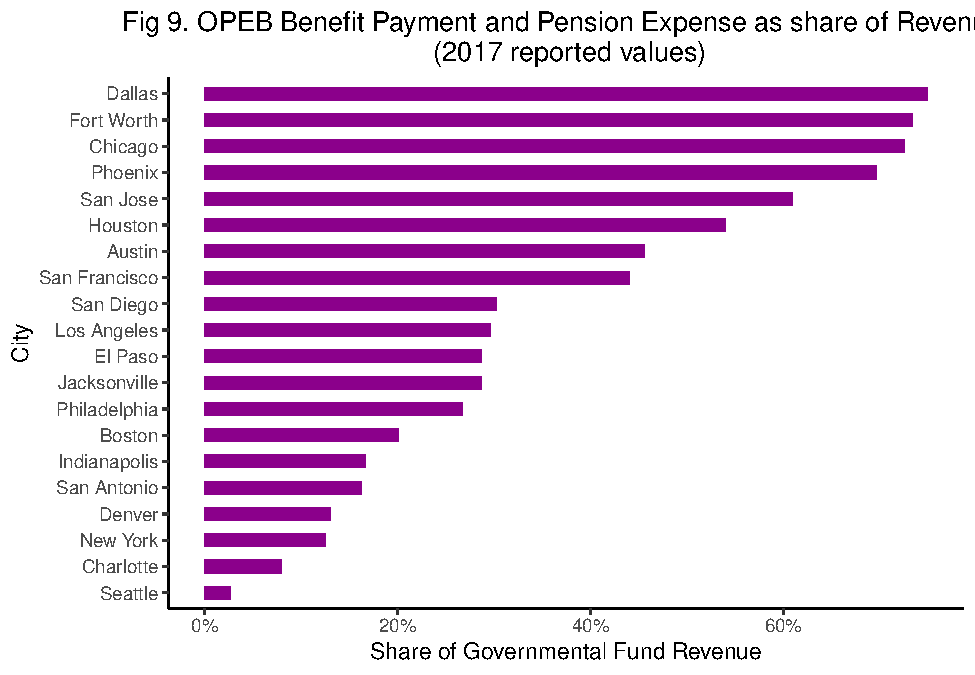
\includegraphics[width=1.2\textwidth]{City-Solvency-Report--Adjusted-_files/figure-latex/unnamed-chunk-14-1.pdf}}%
  %\caption{Caption}
  \label{fig:key}
\end{figure}


\section{Appendix: Methodology, Assumptions, and Data}
\subsection{Discount
Rates}

The unfunded obligations of local cities with regard to pension and OPEB
plans are sensitive to underlying actuarial assumptions, and even small
changes can significantly change reported liabilities. The most
significant of these assumptions is the discount rate.

In 2004, new reporting guidelines from the Governmental Accounting
Standards Board (GASB) were released. These guidelines, which became
effective in 2007, required cities to report for the cost of both OPEB
and Pension plans on an accrual basis. In particular, GASB Statement
No.~45, Accounting and Financial Reporting by Employers for
Post Employment Benefits Other Than Pensions, represented a significant
change towards accrual reporting for governmental entities.

Although GASB 45 was a major shift in governmental accounting and
financial reporting, it still provides an incentive for governments to
use a higher rate to discount future benefit promises if they set up a
trust and commit to paying the Annual Required Contribution (ARC). The
ARC is the minimum amount required to cover both the plan's normal costs
(the Present Value of benefit payments for the current year) and the
unfunded liability (the gap between current assets and the present value
of future benefits already promised to employees) amortized over a
specific period. Thus, it becomes clear that the discount rate plays a
pivotal role in assessing the ARC. In fact, the higher the discount
rate, the lower the ARC, and vice versa.

\begin{figure}[h]
  \makebox[\textwidth][c]{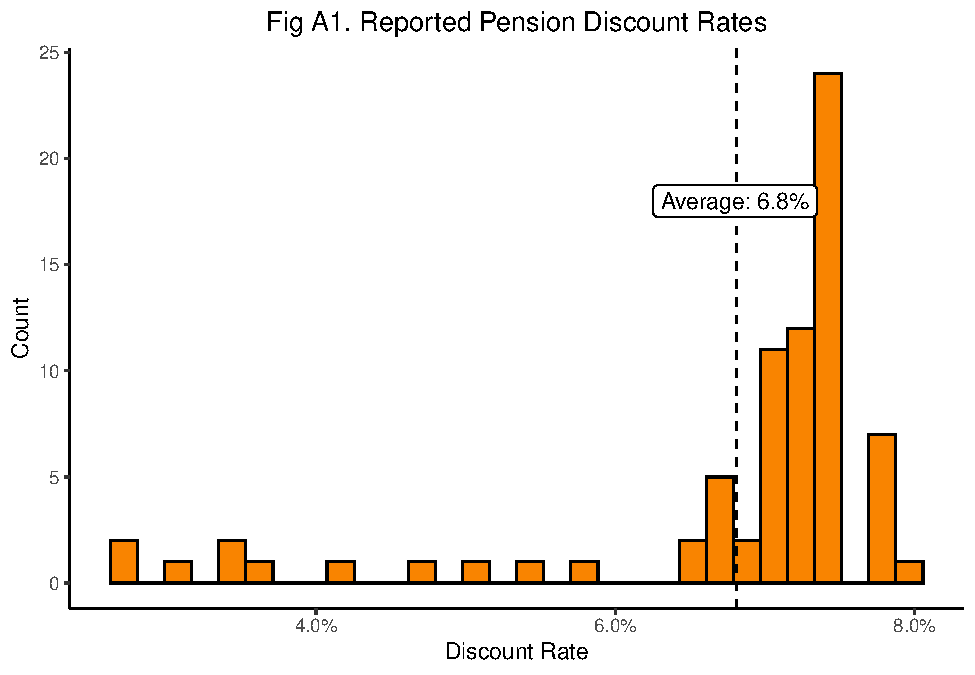
\includegraphics[width=1.2\textwidth]{City-Solvency-Report--Adjusted-_files/figure-latex/unnamed-chunk-15-1.pdf}}%
  %\caption{Caption}
  \label{fig:key}
\end{figure}

\begin{figure}[h]
  \makebox[\textwidth][c]{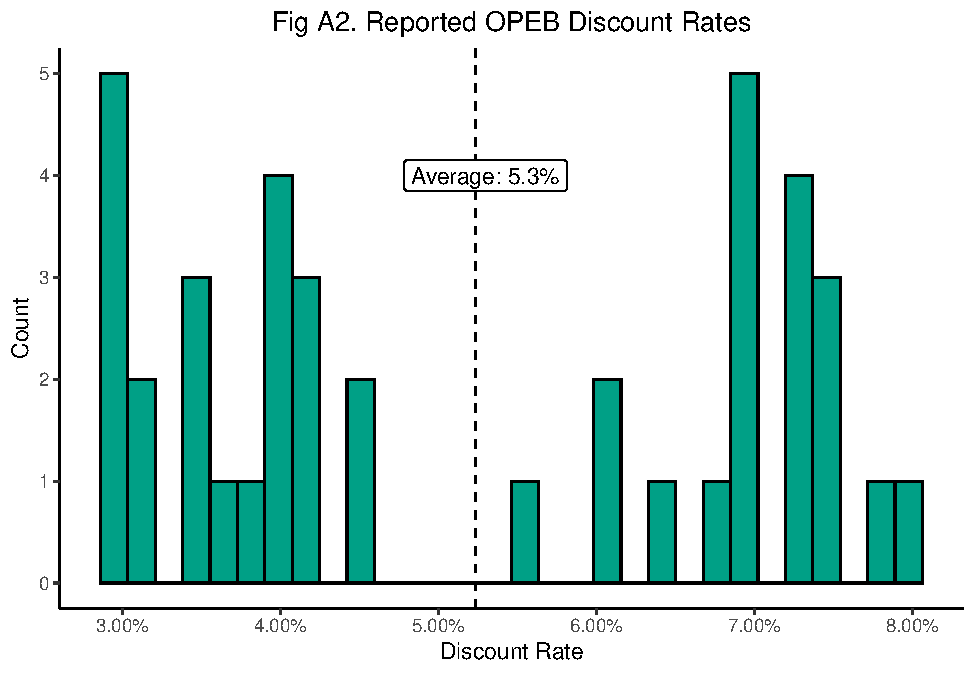
\includegraphics[width=1.2\textwidth]{City-Solvency-Report--Adjusted-_files/figure-latex/unnamed-chunk-15-2.pdf}}%
  %\caption{Caption}
  \label{fig:key}
\end{figure}

In other words, with a trust and a commitment to paying the ARC, cities
can discount obligations by their own estimate of the expected long-term
return of their assets. This idiosyncrasy is what makes it problematic
to compare cities according to their own reports: there is wide
variation in discount rates chosen by cities (and sometimes, even by
departments within cities). For example, for OPEB alone, discount rates
for the plans sponsored by the cities in our report ranged from
\textbf{2.92\%} to \textbf{7.95\%} as displayed in Figure A2.  Pension discount rates, in comparison, range from 2.75\% to 8\% and are somewhat higher on average, cluster more tightly between 6.5\% and 8\%,  but possess a notable left skew (Figure A1).\footnote{Note display discount rates are per plan, not city. Across our data, we have 69 pension plans across our 21 cities and 41 OPEB plans across our 20 cities.}



\subsection{Data Tables}



\begin{table}[h]
\centering
\caption{Total Pension and OPEB Liabilities
(Millions)}
\begin{tabular}{l|l|l|l|l}
\hline
& \multicolumn{2}{c}{Pensions} & \multicolumn{2}{c}{OPEB} \\
\hline
City &  Reported &  Standardized &  Reported &  Standardized\\
\hline
Austin & 6,026.22 & 10,004.34 & 2,004.66 & 2,388.49\\
\hline
Boston & 8,336.25 & 13,635.81 & 4,631.37 & 6,569.90\\
\hline
Charlotte & 2,515.18 & 3,683.47 & 276.34 & 601.85\\
\hline
Chicago & 38,113.11 & 58,716.87 & 842.92 & 842.92\\
\hline
Columbus & 5,621.13 & 9,621.40 & NA & NA\\
\hline
Dallas & 8,908.86 & 14,636.43 & 499.91 & 577.88\\
\hline
Denver & 5,250.93 & 8,611.40 & 41.05 & 47.45\\
\hline
El Paso & 2,633.80 & 4,327.22 & 109.74 & 136.32\\
\hline
Fort Worth & 5,318.31 & 5,395.53 & 717.70 & 853.81\\
\hline
Houston & 16,673.85 & 25,807.01 & 2,153.00 & 2,488.78\\
\hline
Indianapolis & 2,330.36 & 2,906.97 & 203.53 & 216.97\\
\hline
Jacksonville & 6,624.00 & 10,273.60 & 198.60 & 229.57\\
\hline
Los Angeles & 51,929.33 & 82,389.56 & 2,701.59 & 9,937.48\\
\hline
Minneapolis & 3,967.82 & 6,518.97 & 34.81 & 37.43\\
\hline
New York & 195,068.92 & 298,844.08 & 88,422.67 & 90,753.81\\
\hline
Philadelphia & 11,168.43 & 18,868.07 & 2,474.54 & 3,172.48\\
\hline
Phoenix & 8,637.08 & 14,190.38 & 185.54 & 510.68\\
\hline
San Antonio & 7,668.03 & 12,003.96 & 1,043.35 & 2,243.07\\
\hline
San Diego & 9,510.89 & 14,068.23 & 553.87 & 1,026.09\\
\hline
San Francisco & 25,777.96 & 42,352.15 & 4,220.04 & 5,261.79\\
\hline
San Jose & 8,456.99 & 12,739.79 & 1,182.08 & 2,029.43\\
\hline
Seattle & 5,303.11 & 8,550.06 & 702.21 & 763.87\\
\hline
\end{tabular}
\end{table}

\begin{table}[h]
\centering
\caption{Per Capita Pension and OPEB Liabilities}
\begin{tabular}{l|l|l|l|l}
\hline
& \multicolumn{2}{c}{Pensions} & \multicolumn{2}{c}{OPEB} \\
\hline
City &  Reported &  Standardized &  Reported &  Standardized\\
\hline
Austin & 6,338.61 & 10,522.97 & 2,108.59 & 2,512.31\\
\hline
Boston & 12,168.04 & 19,903.56 & 6,760.20 & 9,589.79\\
\hline
Charlotte & 2,927.91 & 4,287.92 & 321.69 & 700.61\\
\hline
Chicago & 14,032.81 & 21,618.88 & 310.36 & 310.36\\
\hline
Columbus & 6,393.68 & 10,943.73 & NA & NA\\
\hline
Dallas & 6,643.45 & 10,914.56 & 372.79 & 430.93\\
\hline
Denver & 7,442.93 & 12,206.24 & 58.18 & 67.25\\
\hline
El Paso & 3,852.96 & 6,330.26 & 160.54 & 199.42\\
\hline
Fort Worth & 6,083.85 & 6,172.19 & 821.01 & 976.71\\
\hline
Houston & 7,208.75 & 11,157.37 & 930.83 & 1,075.99\\
\hline
Indianapolis & 2,670.35 & 3,331.09 & 233.23 & 248.63\\
\hline
Jacksonville & 7,425.49 & 11,516.69 & 222.63 & 257.35\\
\hline
Los Angeles & 12,982.33 & 20,597.39 & 675.40 & 2,484.37\\
\hline
Minneapolis & 9,395.05 & 15,435.69 & 82.42 & 88.63\\
\hline
New York & 22,621.93 & 34,656.63 & 10,254.28 & 10,524.62\\
\hline
Philadelphia & 7,064.15 & 11,934.26 & 1,565.17 & 2,006.63\\
\hline
Phoenix & 5,311.86 & 8,727.17 & 114.11 & 314.07\\
\hline
San Antonio & 5,112.02 & 8,002.64 & 695.57 & 1,495.38\\
\hline
San Diego & 6,697.81 & 9,907.20 & 390.05 & 722.60\\
\hline
San Francisco & 29,148.62 & 47,890.01 & 4,771.84 & 5,949.81\\
\hline
San Jose & 8,171.00 & 12,308.97 & 1,142.11 & 1,960.80\\
\hline
Seattle & 7,317.20 & 11,797.33 & 968.90 & 1,053.99\\
\hline
\end{tabular}
\end{table}

\begin{table}[h]
\centering
\caption{Reported OPEB Benefit Payment and Pension Expense as Share of Government Revenue}
\begin{tabular}{l|l|l|l}
\hline
         City 	&	   Pension 	&	 OPEB 	&	  Overall	\\	\hline
       Austin 	&	40.4	&	5.2	&	45.6	\\	\hline
       Boston 	&	15.1	&	5.0	&	20.1	\\	\hline
    Charlotte 	&	5.4	&	2.6	&	8.0	\\	\hline
      Chicago 	&	70.2	&	2.3	&	72.6	\\	\hline
     Columbus 	&	28.7	&	NA	&	NA	\\	\hline
       Dallas 	&	73.6	&	1.3	&	74.9	\\	\hline
       Denver 	&	12.9	&	0.2	&	13.1	\\	\hline
      El Paso 	&	27.4	&	1.3	&	28.7	\\	\hline
  Fort Worth  	&	68.7	&	4.7	&	73.4	\\	\hline
      Houston 	&	52.4	&	1.7	&	54.0	\\	\hline
 Indianapolis 	&	16.4	&	0.3	&	16.7	\\	\hline
 Jacksonville 	&	28.2	&	0.5	&	28.7	\\	\hline
  Los Angeles 	&	22.4	&	7.2	&	29.6	\\	\hline
    New York  	&	9.6	&	2.9	&	12.5	\\	\hline
 Philadelphia 	&	22.3	&	4.4	&	26.7	\\	\hline
      Phoenix 	&	67.2	&	2.5	&	69.7	\\	\hline
  San Antonio 	&	11.0	&	5.2	&	16.2	\\	\hline
    San Diego 	&	28.2	&	2.1	&	30.3	\\	\hline
San Francisco 	&	40.1	&	4.0	&	44.1	\\	\hline
     San Jose 	&	54.5	&	6.5	&	61.0	\\	\hline
      Seattle 	&	0.9	&	1.8	&	2.7	\\	\hline
\end{tabular}
\end{table}


\end{document}


\subsection{City Plans}

Estimating city pension and OPEB obligations is complicated not just by the assumptions of discount rates, but also by certain vagarities in what financial obligations cities themselves are ultimately responsible for.  Cities often have multiple plans for different city services - the police may be covered by one pension plan, municipal employees by another, teachers by another, etc. Sometimes certain classes of employees are employed directly by the city, while other times, those employees may be technically employed by component units of the city. Sometimes cities take part in broader regional pension or OPEB plans, and may be considered to have partial responsibility for those plans, as well. We follow the city's CAFR in defining their obligations. The following tables show what plans we include for each city in our analysis, as well as the proportion of responsibility the city was considered to own for each plan. In the case of non-full obligations, proportions given are sourced from city financial documents.

\begin{table}[h]
\centering
\caption{City Pension Plans Under Consideration, A-J}
\begin{tabular}{l|l|l}
\hline
City	&	Entity/Source	&	Obligation	\\
\hline
Austin	&	City Employees	&	1	\\
Austin	&	Police Officers	&	1	\\
Austin	&	Fire Fighters	&	1	\\
Boston	&	BRS-Excluding Teachers	&	1	\\
Charlotte	&	LGERS	&	0.06115	\\
Charlotte	&	LGERS	&	0.00241	\\
Charlotte	&	System	&	1	\\
Charlotte	&	LEOSSA	&	1	\\
Chicago	&	Municipal Employees'	&	1	\\
Chicago	&	Laborers'	&	1	\\
Chicago	&	Policemen’s	&	1	\\
Chicago	&	Firemen's	&	1	\\
Columbus	&	OP\&F	&	0.1545	\\
Columbus	&	OPERS	&	0.023	\\
Dallas	&	ERF	&	1	\\
Dallas	&	Combined Plan	&	1	\\
Dallas	&	Supplemental Plan	&	1	\\
Denver	&	DERP	&	0.907	\\
Denver	&	FPPA SWDB	&	0.395074604	\\
Denver	&	PERA SDTF	&	0.00008	\\
Denver	&	PERA JDTF	&	0.0601	\\
Denver	&	FPPA Old Hire Fire	&	1	\\
Denver	&	FPPA Old Hire Police	&	1	\\
El Paso	&	CERT	&	0.801	\\
El Paso	&	CERT	&	0.191	\\
El Paso	&	FPPF-Firemen Division	&	1	\\
El Paso	&	FPPF-Policemen Division	&	1	\\
Fort Worth 	&	Pensions	&	1	\\
Houston	&	HMEPS	&	1	\\
Houston	&	HRRFP	&	1	\\
Houston	&	HPOPS	&	1	\\
Indianapolis	&	Pre-1977 Police Plan	&	1	\\
Indianapolis	&	Pre-1977 Fire Plan	&	1	\\
Indianapolis	&	1977 Police and Firefighters' Plan	&	0.229	\\
Indianapolis	&	PERF	&	0.0136	\\
Jacksonville	&	General Employee Pension Plan	&	1	\\
Jacksonville	&	Corrections Officers Pension Plan	&	1	\\
Jacksonville	&	Police and Fire Pension Plan	&	1	\\
\hline
\end{tabular}
\end{table}

\begin{table}[h]
\centering
\caption{City Pension Plans Under Consideration, L-Z}
\begin{tabular}{l|l|l}
\hline
City	&	Entity/Source	&	Obligation	\\
\hline
Los Angeles	&	Pensions	&	1	\\
Los Angeles	&	LACERS	&	1	\\
Los Angeles	&	DWP Plans	&	1	\\
%Minneapolis	&	GERF	&	0.052275	\\
%Minneapolis	&	GERF	&	0.00938	\\
%Minneapolis	&	GERF	&	0.00857	\\
%Minneapolis	&	PEPFF	&	0.208345	\\
%Minneapolis	&	PEPFF	&	0.003266	\\
%Minneapolis	&	TRA	&		\\
New York 	&	POLICE	&	1	\\
New York 	&	FIRE	&	1	\\
New York 	&	NYCERS	&	0.5433	\\
New York 	&	TRS	&	0.9762	\\
New York 	&	BERS	&	0.9996	\\
Philadelphia	&	the Fund	&	0.9709	\\
Philadelphia	&	the Fund	&	0.0263	\\
Philadelphia	&	the Fund	&	0.0004	\\
Philadelphia	&	the Fund	&	0.00024	\\
Phoenix	&	COPERS	&	1	\\
Phoenix	&	Police - PSPRS	&	1	\\
Phoenix	&	Fire - PSPRS	&	1	\\
San Antonio	&	City - TMRS	&	1	\\
San Antonio	&	Fire and Police Pension Plan	&	1	\\
San Antonio	&	CPS Energy All Employee Plan	&	1	\\
San Antonio	&	SAWS-TMRS	&	1	\\
San Antonio	&	SAWS Retirement Plan	&	1	\\
San Antonio	&	District Special Project Retirement Income Plan	&	1	\\
San Diego	&	SDCERS	&	1	\\
San Francisco	&	SFERS	&	0.940674	\\
San Jose	&	PFDRP	&	1	\\
San Jose	&	FCERS	&	1	\\
Seattle	&	SCERS	&	1	\\
Seattle	&	Firemen’s Pension Fund	&	1	\\
Seattle	&	Police Relief and Pension Fund	&	1	\\
Seattle	&	LEOFF Plan 1	&	0.0355	\\
Seattle	&	LEOFF Plan 2	&	0.0917	\\
\hline
\end{tabular}
\end{table}

\begin{table}[h]
\centering
\caption{OPEB Plans Under Consideration, L-Z}
\begin{tabular}{l|l }
\hline
City	&	Entity/Source	\\
\hline
Austin	&	City	\\
Boston	&	Primary Government	\\
Boston	&	Public Health Commission	\\
Boston	&	MBTA Transit Authority	\\
Charlotte	&	City	\\
Chicago	&	Retiree Settlement Health Plan	\\
Chicago	&	Special Benefits (Police \& Fire)	\\
Columbus	&	City	\\
Dallas	&	City	\\
Denver	&	FPPA (Fire \& Police)	\\
El Paso	&	City	\\
Fort Worth	&	Healthcare	\\
Fort Worth	&	Death Benefit	\\
Houston	&	City	\\
Indianapolis	&	City	\\
Jacksonville	&	City	\\
Los Angeles	&	Primary Government	\\
Los Angeles	&	LACERS City Employee Retirement System	\\
Los Angeles	&	DWP Department Water and Power	\\
Minneapolis	&	City	\\
New York	&	City	\\
Philadelphia	&	Primary Government	\\
Philadelphia	&	SDP School District of Philadelphia 	\\
Philadelphia	&	Philadelphia Gas Work	\\
Phoenix	&	MERP (Medical Reimbursment Plan)	\\
Phoenix	&	LTD (Long Term Disability)	\\
San Antonio	&	Primary Government	\\
San Antonio	&	Fire \& Police	\\
San Antonio	&	CPS Energy Health (City Public Service)	\\
San Antonio	&	CPS Energy Life (City Public Service)	\\
San Antonio	&	CPS Energy Disability (City Public Service)	\\
San Antonio	&	SAWS (Water System)	\\
San Diego	&	City	\\
San Francisco	&	Retiree Health Care Trust Fund	\\
San Francisco	&	Transportation Authority (County)	\\
San Francisco	&	Successor Agency	\\
San Jose	&	PFDRP (Police \& Fire)	\\
San Jose	&	FCERS (City Employees)	\\
Seattle	&	Primary Government	\\
Seattle	&	Firemen Plan	\\
Seattle	&	Police Relief Plan	\\
\hline
\end{tabular}
\end{table}

